\documentclass{beamer}

\usepackage{amsmath}
\usepackage{amsfonts}
\usepackage{physics}
\usepackage{bm} 
\usepackage{graphicx}

\title{Finite Element Analysis of Electromagnetic Waves in Anisotropic Media}
\author{
    Syed Khalid 21BEE1288 \\
    S. Aditya  21BEE1094 \\
    Niraj Kumar Yadav  21BEE1295 \\
    Under the Guidance of \\ Dr. Mohamed Imran A, Associate Professor 
  }
\institute{
    Course Code: EEE497J  \\
    School: SELECT \\
    VIT Chenna
}
\date{}
\begin{document}

\begin{frame}
  \titlepage
\end{frame}
% Slide 2 - Introduction to FEM
\begin{frame}{Introduction to Finite Element Method}
    \begin{itemize}
        \item \textbf{What is FEM?}
        \begin{itemize}
            \item A numerical technique for solving differential equations in engineering and mathematical models.
        \end{itemize}
        \item \textbf{Applications:}
        \begin{itemize}
            \item Structural analysis
            \item Heat transfer
            \item Fluid dynamics
            \item Electromagnetics
        \end{itemize}
        \item \textbf{Key Idea:} Break down a complex domain into smaller, simpler parts (elements), and solve locally.
    \end{itemize}
\end{frame}

% Slide 3 - Steps in FEM

% Slide 4 - Key Concepts in FEM
\begin{frame}{Key Concepts in FEM}
    \begin{itemize}
        \item \textbf{Meshing:} Divide the domain into finite elements.
        \item \textbf{Shape Functions:} Local functions that approximate the solution over each element.
        \item \textbf{Stiffness Matrix:} Matrix representation of the system based on element contributions.
        \item \textbf{Boundary Conditions:} Ensure physical accuracy of the model.
    \end{itemize}
\end{frame}

% Slide 5 - Advantages and Limitations of FEM
\begin{frame}{Advantages and Limitations of FEM}
    \begin{itemize}
        \item \textbf{Advantages:}
        \begin{itemize}
            \item Handles complex geometries and boundary conditions.
            \item Provides local accuracy through adaptive meshing techniques thus capturing local effects.
            \item Easily incorporates non-linear material properties thus suitable for anisotropic media.
            \item Allows for efficient parallel processing and distributed computing.
        \end{itemize}
        \item \textbf{Limitations:}
        \begin{itemize}
            \item Computationally intensive, particularly for large-scale models.
            \item Solution accuracy depends on mesh quality and element size.
            \item Requires significant memory for storing large stiffness matrices.
        \end{itemize}
    \end{itemize}
\end{frame}


\begin{frame}{Steps in FEM}
    \begin{enumerate}
        \item \textbf{Discretization}
        \begin{itemize}
            \item Divide the domain into small elements (meshing).
            \item Types of elements: Triangular, Quadrilateral, etc.
        \end{itemize}
        \item \textbf{Interpolation}
        \begin{itemize}
            \item Approximate the solution over each element using shape functions.
        \end{itemize}
        \item \textbf{Formulation}
        \begin{itemize}
            \item Set up governing equations (e.g., weak form of the differential equation).
            \item Construct a global system from local contributions.
        \end{itemize}
    \end{enumerate}
\end{frame}

% Slide 2 - Governing Differential Equation
\begin{frame}{Step 1: Governing Differential Equation}
    The problem is defined by a partial differential equation (PDE):
    \[
    \mathcal{L}(u) = f \quad \text{in} \quad \Omega
    \]
    where:
    \begin{itemize}
        \item \( \mathcal{L} \) is the differential operator (e.g., Laplace, Helmholtz).
        \item \( f \) is the source term.
        \item \( \Omega \) is the domain.
    \end{itemize}
    \textbf{Example: Poisson equation in 1D}
    \[- u'' = f, \Omega = (0,1) \]
\end{frame}

% Slide 3 - Weak Formulation of the PDE
\begin{frame}{Step 2: Weak Formulation of the PDE}
    Convert the PDE into its weak form:
    \[
    \int_\Omega v \mathcal{L}(u) \, d\Omega = \int_\Omega v f \, d\Omega
    \]
    Apply integration by parts to reduce the order of derivatives:
    \[
    \int_\Omega \nabla v \cdot \mathbf{k} \nabla u \, d\Omega = \int_\Omega v f \, d\Omega
    \]
    where \( v \) is a test function.
\end{frame}

% Slide 4 - Discretization (Meshing)
\begin{frame}{Step 3: Discretization (Meshing)}
    The domain \( \Omega \) is divided into smaller, simpler elements:
    \begin{itemize}
        \item Triangular or quadrilateral elements in 2D.
        \item Tetrahedral or hexahedral elements in 3D.
    \end{itemize}
    Each element contains nodes where the solution is approximated. The number of nodes is denoted as \( N \).

  \begin{figure}
    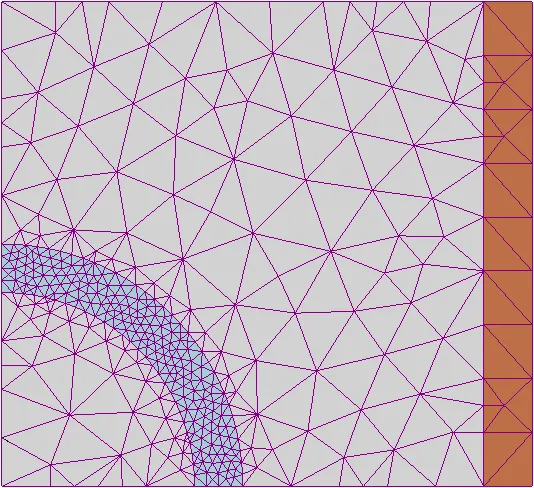
\includegraphics[width=0.3\textwidth]{mesh.png}
    \caption{Example of triangular mesh in 2D}
  \end{figure}
\end{frame}

% Slide 5 - Approximation of the Solution
\begin{frame}{Step 4: Approximation of the Solution}
    Approximate the solution \( u(\mathbf{x}) \) using shape functions:
    \[
    u(\mathbf{x}) \approx \sum_{i=0}^{N} u_i N_i(\mathbf{x})
    \]
    where:
    \begin{itemize}
        \item \( u_i \) are the nodal values.
        \item \( N_i(\mathbf{x}) \) are shape functions (e.g., polynomials).
    \end{itemize}
    The test function \( v \) is also approximated using the same shape functions.

  \begin{figure}
    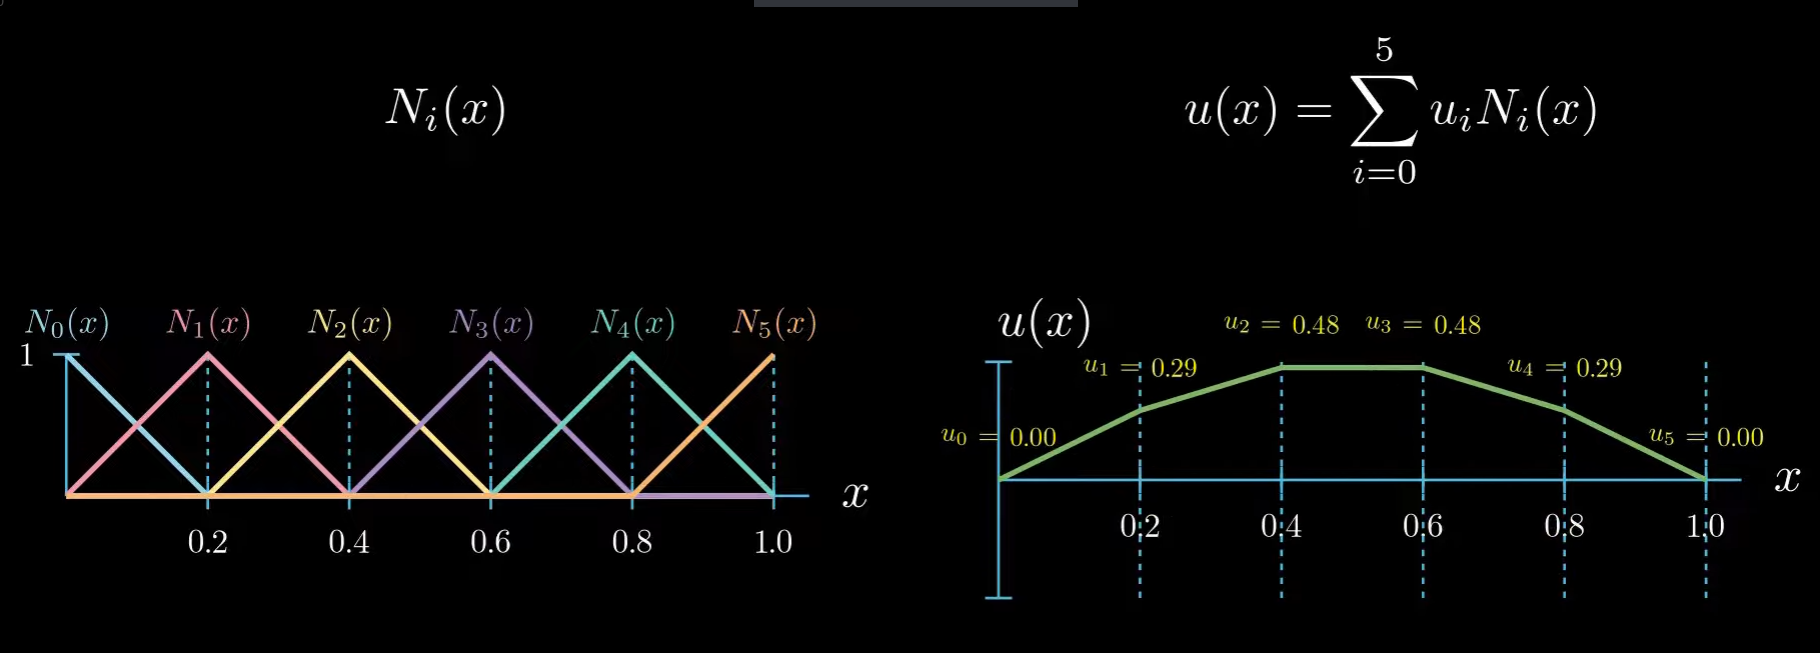
\includegraphics[width=0.8\textwidth]{shape.png}
    \caption{a univariate function approximated by simple shape functions }
  \end{figure}
\end{frame}

% Slide 6 - Assembly of the Elemental System
\begin{frame}{Step 5: Assembly of the Elemental System}
    Substitute the shape functions into the weak form. For each element, we get a system of equations:
    \[
    \sum_{e} \int_{\Omega_e} \nabla N_j \cdot \mathbf{k} \nabla N_i \, d\Omega_e = \sum_{e} \int_{\Omega_e} N_j f \, d\Omega_e
    \]
    The global system is:
    \[
    \mathbf{K} \mathbf{U} = \mathbf{F}
    \]
    where \( \mathbf{K} \) is the stiffness matrix, \( \mathbf{U} \) is the vector of nodal values, and \( \mathbf{F} \) is the load vector.
\end{frame}

% Slide 7 - Imposing Boundary Conditions
\begin{frame}{Step 6: Imposing Boundary Conditions}
    Apply boundary conditions to the system:
    \begin{itemize}
        \item \textbf{Dirichlet boundary conditions:} Known values of \( u \) at the boundary.
        \item \textbf{Neumann boundary conditions:} Known flux \( \mathbf{k} \nabla u \cdot \hat{n} \) at the boundary.
    \end{itemize}
    Modify the global stiffness matrix and load vector accordingly.
\end{frame}

% Slide 8 - Solve the System of Equations
\begin{frame}{Step 7: Solve the System of Equations}
    Solve the algebraic system:
    \[
    \mathbf{K} \mathbf{U} = \mathbf{F}
    \]
    \begin{itemize}
        \item Use \textbf{direct solvers} (e.g., Gaussian elimination) for small systems.
        \item Use \textbf{iterative solvers} (e.g., Conjugate Gradient) for large systems.
    \end{itemize}
\end{frame}

% Slide 9 - Post-Processing
\begin{frame}{Step 8: Post-Processing}
    After solving for \( \mathbf{U} \), the solution can be:
    \begin{itemize}
        \item \textbf{Interpolated} within elements using the shape functions.
        \item Compute \textbf{derived quantities} such as fluxes and gradients.
    \end{itemize}
    Example: In electromagnetics, compute the electric or magnetic field from the solution \( u \).
\end{frame}


\begin{frame}{Simulation with FEniCS}

FEniCS is a popular open-source computing platform for solving partial differential equations (PDEs) with the finite element method (FEM). FEniCS enables users to quickly translate scientific models into efficient finite element code. \\

We are using its high level Python interface. 

  Basic workflow: 
  \begin{itemize}
    \item Define the mesh and function spaces.
    \item Formulate the problem (weak form).
    \item Solve using FEM.
  \end{itemize}

        \href{https://fenicsproject.org}{FEniCS Website}
\end{frame}

\begin{frame} {Maxwell's equations in the differential form:}
\begin{align*}
    \nabla \cdot \mathbf{E} &= \frac{\rho}{\varepsilon_0}, &\nabla \cdot \mathbf{B} &= 0 \\
    \nabla \times \mathbf{E} &= -\frac{\partial \mathbf{B}}{\partial t}, &\nabla \times \mathbf{H} &= \mathbf{J} + \frac{1}{\mu_0}\frac{\partial \mathbf{E}}{\partial t}
\end{align*}


\begin{itemize}
    \item \(\mathbf{E}\): Electric field vector, representing the force per unit charge.
    \item \(\mathbf{B}\): Magnetic field vector, related to the magnetic influence on moving charges and currents.
    \item \(\mathbf{H}\): Magnetic field intensity vector, related to the magnetic field \(\mathbf{B}\) by the relation \(\mathbf{B} = \mu_0 \mathbf{H}\) in free space.
    \item \(\rho\): Electric charge density, representing the amount of charge per unit volume.
    \item \(\mathbf{J}\): Electric current density vector, representing the current per unit area.
    \item \(\varepsilon_0\): Permittivity of free space, \(\varepsilon_0 = 8.854 \times 10^{-12} \, \mathrm{F/m}\) (farads per meter).
    \item \(\mu_0\): Permeability of free space, \(\mu_0 = 4\pi \times 10^{-7} \, \mathrm{H/m}\) (henries per meter).
\end{itemize}
  
\end{frame}

\begin{frame}{Deriving Electromagnetic Waves from Maxwell's Equations}

\vspace{1em}
\textbf{Step 1: Set Free Space Conditions}
\begin{itemize}
    \item No free charges (\(\rho = 0\))
    \item No free currents (\(\mathbf{J} = 0\))
\end{itemize}

\vspace{1em}
\textbf{Step 2: Take the Curl of Faraday's Law}
\[
\nabla \times \nabla \times \mathbf{E} = -\frac{\partial}{\partial t} (\nabla \times \mathbf{B})
\]

\vspace{0.5em}
Using Ampere's Law:
\[
\nabla \times \mathbf{B} = \frac{1}{\mu_0} \frac{\partial \mathbf{E}}{\partial t}
\]

\textbf{Step 3: Apply Vector Identity}
\[
\nabla \times (\nabla \times \mathbf{E}) = \nabla (\nabla \cdot \mathbf{E}) - \nabla^2 \mathbf{E}
\]
In free space, \(\nabla \cdot \mathbf{E} = 0\), so we get:
\[
-\nabla^2 \mathbf{E} = \mu_0 \varepsilon_0 \frac{\partial^2 \mathbf{E}}{\partial t^2}
\]
\end{frame}
\begin{frame}

\vspace{1em}
\textbf{Result: Wave Equation for \(\mathbf{E}\)}
\[
\nabla^2 \mathbf{E} = \mu_0 \varepsilon_0 \frac{\partial^2 \mathbf{E}}{\partial t^2}
\]

Similarly, we can derive the wave equation for \(\mathbf{B}\):
\[
\nabla^2 \mathbf{B} = \mu_0 \varepsilon_0 \frac{\partial^2 \mathbf{B}}{\partial t^2}
\]

\textbf{Conclusion:} The electric and magnetic fields propagate as waves with velocity \( c = \frac{1}{\sqrt{\mu_0 \varepsilon_0}} \), where \(c\) is the speed of light.
\end{frame}

\begin{frame}{Anisotropic Media}
  \begin{itemize}
    \item Anisotropic media are materials whose properties differ based on direction.
    \item Example: Crystals, certain composites.
    \item They affect how electromagnetic waves propagate, reflecting different velocities in different directions.
  \end{itemize}
  Constitutive relations in anisotropic media:
  \begin{align*}
    \mathbf{D} &= \varepsilon \mathbf{E} \quad \text{(Electric displacement)} \\
    \mathbf{B} &= \mu \mathbf{H} \quad \text{(Magnetic flux density)}
  \end{align*}
  where the permittivity $\varepsilon$ and permeability $\mu$ are tensors:
  \begin{align*}
    \varepsilon_{ij}, \mu_{ij}
  \end{align*}
\end{frame}


\begin{frame}{Challenges}
    \begin{itemize}
        \item \textbf{1. Find the Modified Wave Equation in Anisotropic Medium}
        \begin{itemize}
            \item Identify the governing equations that describe wave propagation in an anisotropic medium.
            \item Consider the material properties that influence the wave behavior, such as permittivity and permeability.
        \end{itemize}
        
        \item \textbf{2. Derive its Weak Formulation}
        \begin{itemize}
            \item Apply the variational principle to convert the modified wave equation into its weak form.
            \item Choose suitable test functions and integrate the equation over the domain.
            \item Incorporate boundary conditions to ensure a well-posed problem.
        \end{itemize}

        \item \textbf{3. Identify Suitable Mesh Schema}
        \begin{itemize}
            \item Analyze the geometry of the problem to determine an appropriate mesh type .
            \item Ensure mesh quality to maintain accuracy and stability in the numerical solution.
        \end{itemize}

        \item \textbf{4. Code Implementation}
    \end{itemize}
\end{frame}




\end{document}
